\chapter{Discussion}\label{chap:discussion}


\subsection{\textbf{Creating the LSTM models}}
% We do not need this because, it wan belongs to first lab.


   \textbf{Makemodel.py} script is used for creating data models. It splits the data in 3 different segments (train, validate, final).
   On the line of code 134, the samples are randomized with \textbf{for} loop. However, there are certain issues regarding this code. 
   Library \textbf{Keras} that is imported in myutils.py file is causing a build error. 
   Keras package is now \textbf{included} in previous installation of tensorflow package. 
   Therefore, imports needed to be adjusted accordingly. 
   "from keras.datasets import imdb" is now "tensorflow.keras.datasets". 
   Also, we need to install all necessary packages (gensim, sklearn, tensorflow). 
   Next, datasets are created using word2vec models created in previous exercise. 
   Unfortunately, new error occurs where we need to adjust 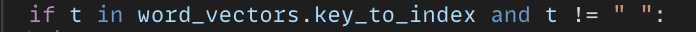
\includegraphics[width=0.5\linewidth]{Screenshot 2024-05-12 at 13.10.36.png} this line of code to match the new key to index parameter. 
   Console is clear from errors so we can proceed to make our new vulnerability model. 
   After loading the data, script creates new training dataset 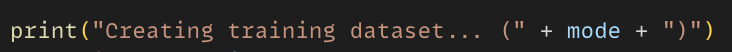
\includegraphics[width=0.5\linewidth]{Screenshot 2024-05-12 at 13.14.57.png}, followed by 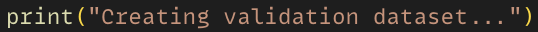
\includegraphics[width=0.5\linewidth]{Screenshot 2024-05-12 at 13.16.00.png} and finally 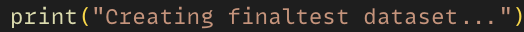
\includegraphics[width=0.5\linewidth]{Screenshot 2024-05-12 at 13.16.43.png}.
                 
   
   %   \begin{figure}
   %     \centering
   %     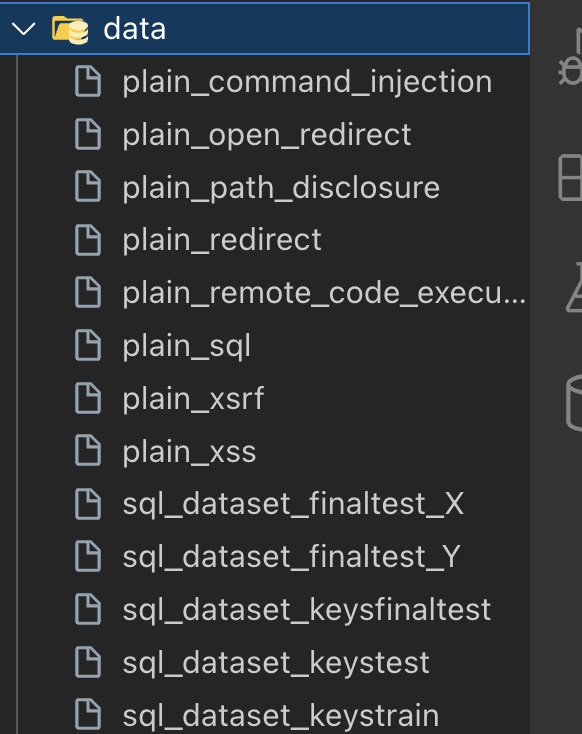
\includegraphics[width=0.5\linewidth]{Screenshot 2024-05-12 at 12.41.42.png}
   %     \caption{Folder structure with data}
   %     \label{fig:enter-label}
   % \end{figure}                               


  % add the console output of final steps
  % adjust the images
  % format the document 
   
   